\documentclass{article}

\usepackage{graphicx}
\usepackage{booktabs}
\usepackage{longtable}
\usepackage{tabu}
\usepackage{listings}
\usepackage{hyperref}
\usepackage{tcolorbox}

\setlength\parindent{0pt}

\title{Baseline Method}

\author{%
devansh
}

\begin{document}

\maketitle

\section{Section 1}

\begin{figure}[!htb]
\minipage{0.49\textwidth}
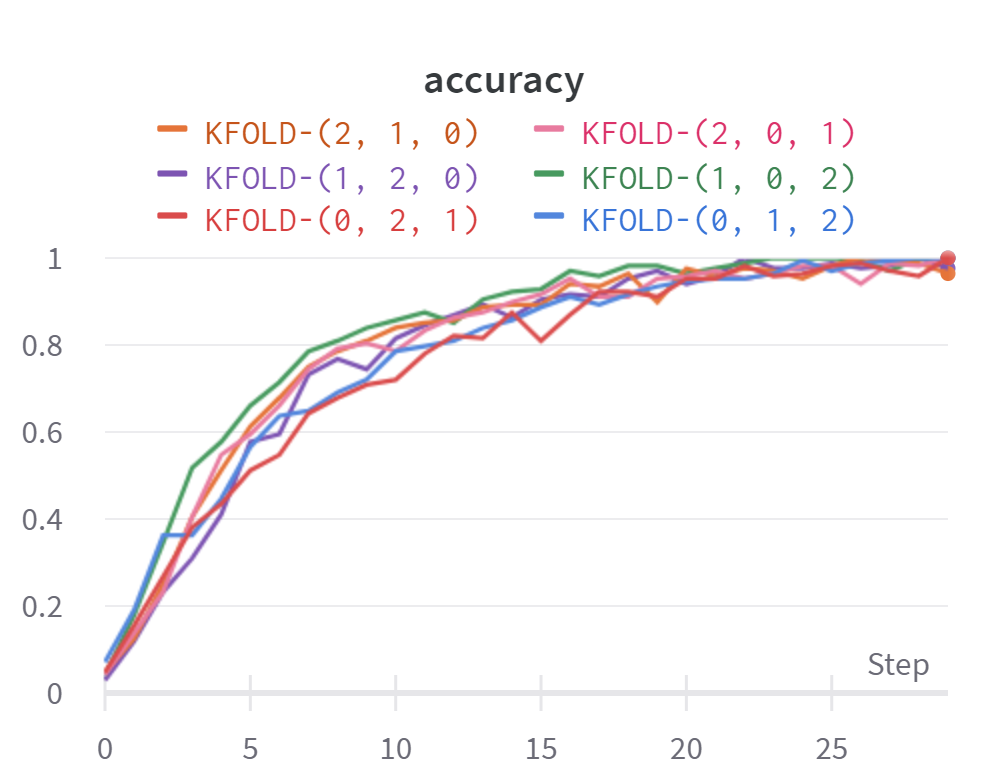
\includegraphics[width=\linewidth]{charts/Section-2-Panel-0-bktx111zt}
\caption{}
\endminipage\hfill
\minipage{0.49\textwidth}
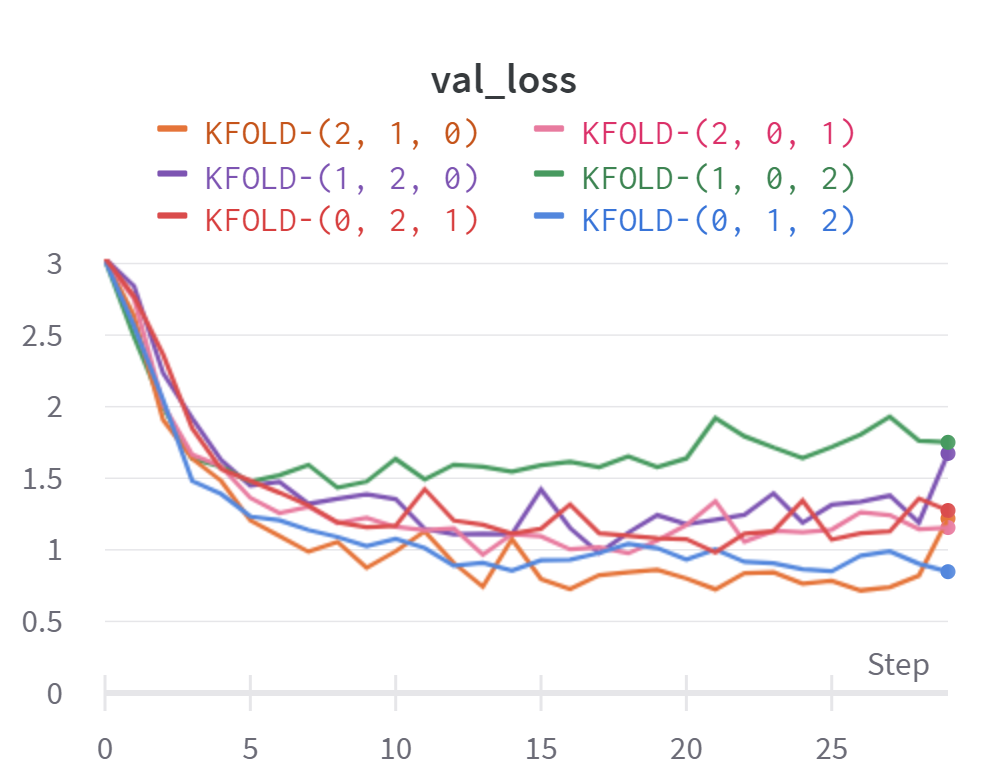
\includegraphics[width=\linewidth]{charts/Section-2-Panel-1-dvjr1ljh0}
\caption{}
\endminipage
\end{figure}

\begin{figure}[!htb]
\minipage{0.49\textwidth}
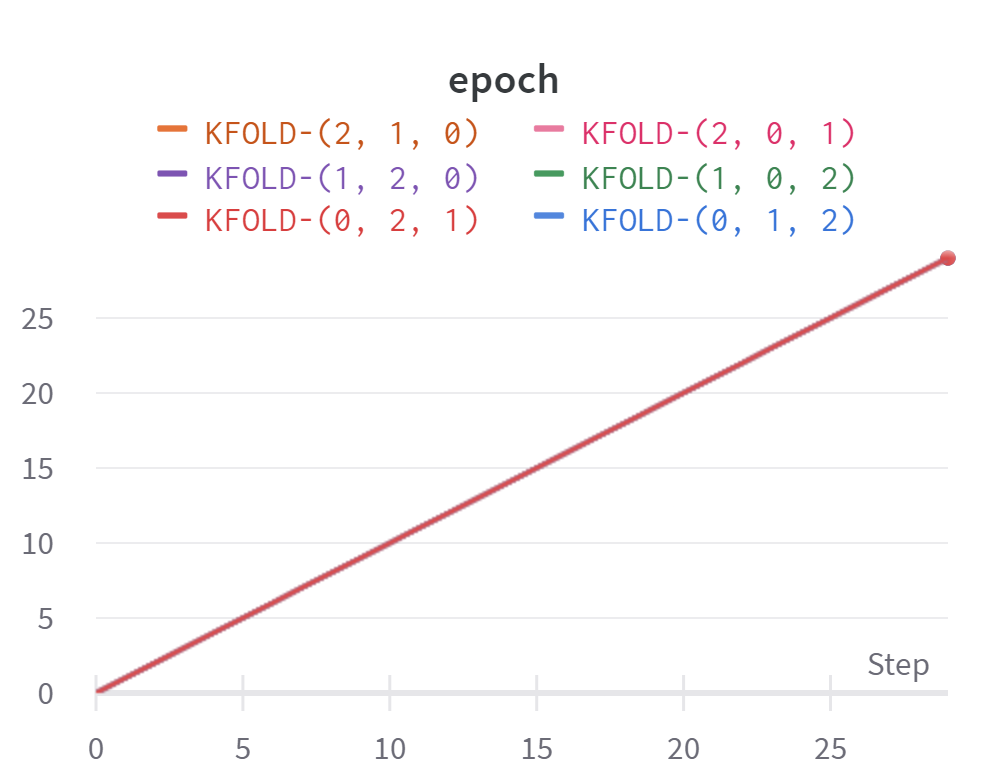
\includegraphics[width=\linewidth]{charts/Section-2-Panel-2-ai3xry1gl}
\caption{}
\endminipage\hfill
\minipage{0.49\textwidth}
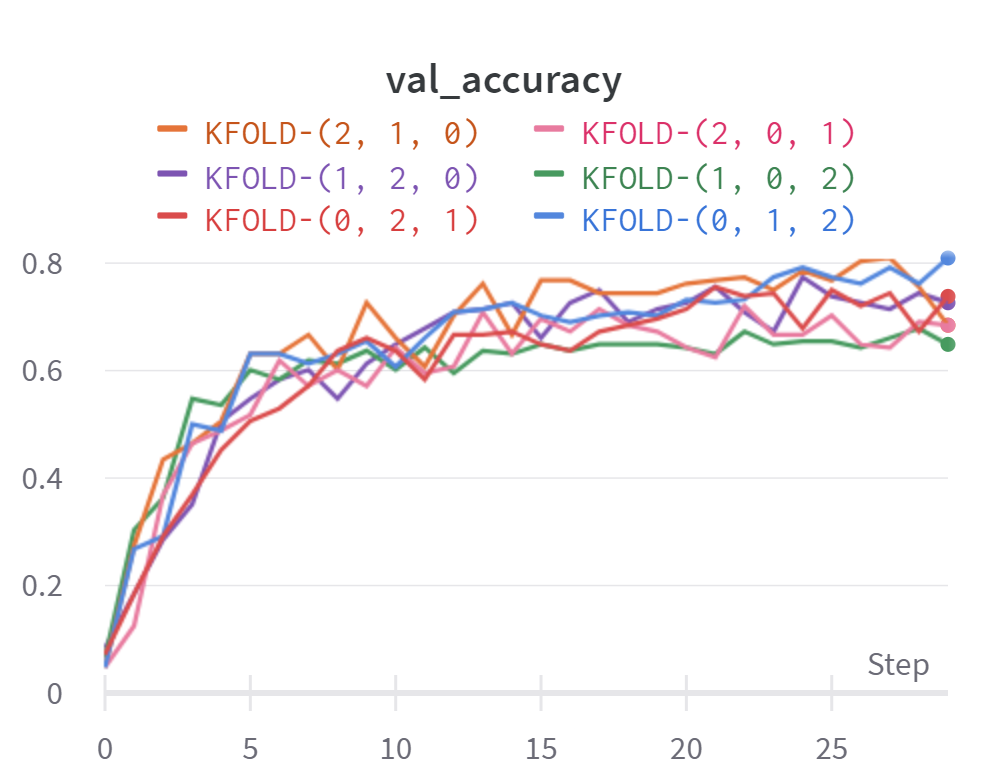
\includegraphics[width=\linewidth]{charts/Section-2-Panel-3-fr749yccp}
\caption{}
\endminipage
\end{figure}

\begin{figure}[!htb]
\minipage{0.49\textwidth}
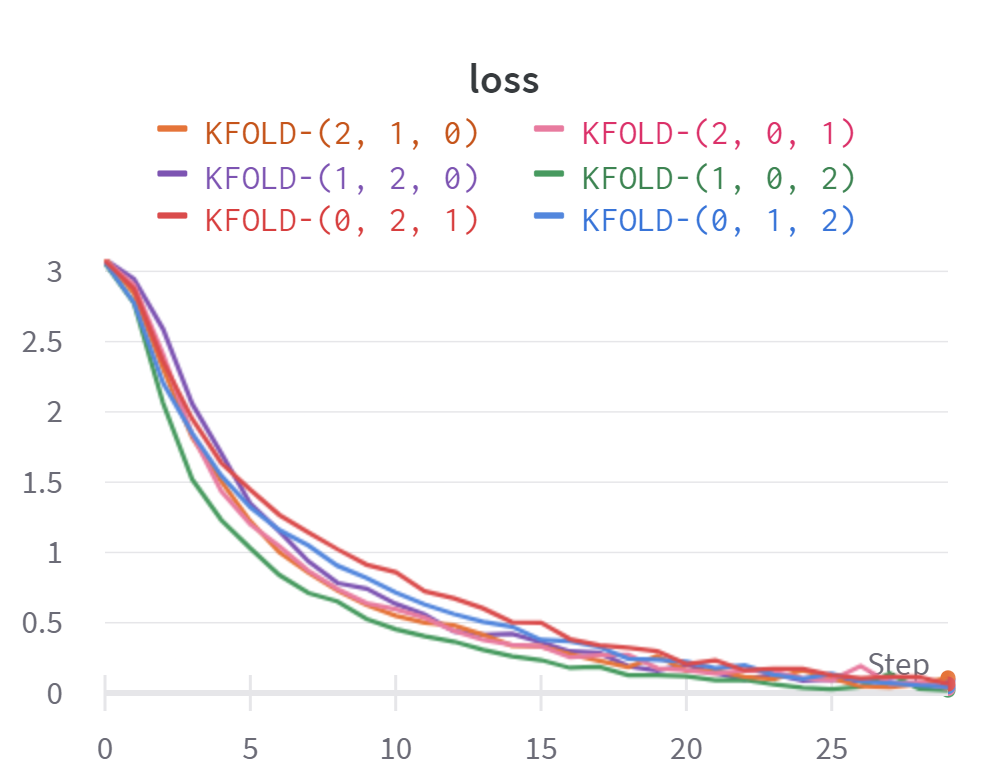
\includegraphics[width=\linewidth]{charts/Section-2-Panel-4-2ibss91a8}
\caption{}
\endminipage
\end{figure}

\nocite{*}
\bibliographystyle{unsrt}
\bibliography{bibliography}
\end{document}